\chapter{Estado da Arte}\label{cap:estado-arte}
Este capítulo revê o trabalho já feito nas duas tarefas em que a dissertação se foca, o reconhecimento do número da camisola e a atribuição da equipa de cada jogador. Antes de as abordar em detalhe, enquadra-se cada tarefa no \emph{pipeline} geral da reconstrução do estado de jogo e apresentam-se as métricas usadas, que servem tanto para avaliar o sistema completo como cada tarefa por si só. A revisão segue por temas, e não trabalho a trabalho, para clarificar as principais linhas de investigação e onde ainda falham.

\section{Reconstrução do Estado de Jogo}\label{sec:sistemas_gsr}

A reconstrução do estado de jogo, proposta por \citet{somers2024soccernet}, é uma tarefa de análise automática de vídeo desportivo, em particular no futebol. Os autores apresentaram a formulação do problema e disponibilizaram o \emph{dataset} SoccerNet-GSR e a arquitetura de referência. Na prática, o objetivo é converter um vídeo de uma única câmara, \emph{frame} a \emph{frame}, numa projeção bidimensional do terreno de jogo (Figura~\ref{fig:gsr-minimap}). Esta transformação implica detetar cada interveniente e acompanhá-lo ao longo do vídeo, localizar as linhas do campo para o situar no terreno e, por fim, identificar a equipa, a função e o número da camisola de cada um.

\begin{figure}[H]
    \centering
    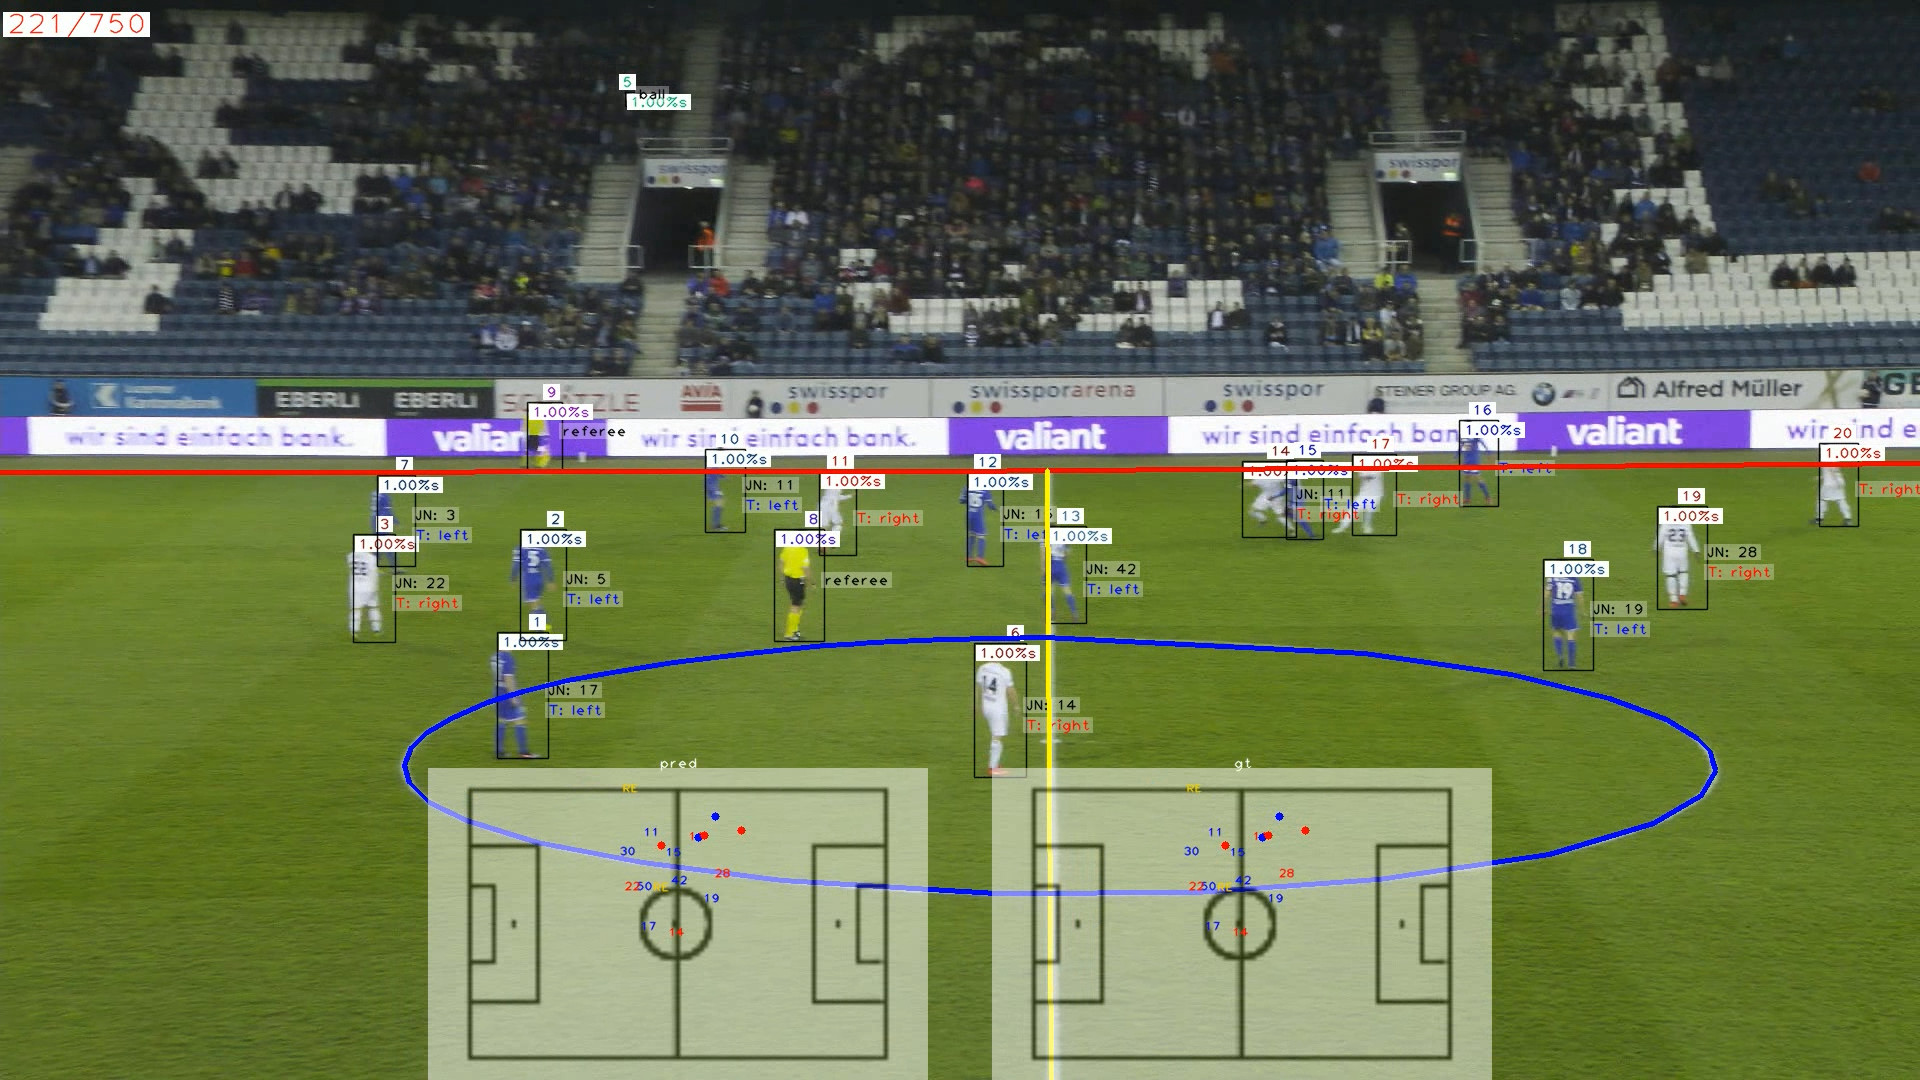
\includegraphics[width=0.8\textwidth]{gamestate-example.jpg}
    \caption{Exemplo de reconstrução do estado de jogo, com a posição, a equipa e o número da camisola projetados num mapa bidimensional do campo. Adaptado de \citet{somers2024soccernet}.}
    \label{fig:gsr-minimap}
\end{figure}

O \emph{dataset} SoccerNet-GSR é composto por sequências de 30 segundos, extraídas de transmissões televisivas de jogos profissionais. Cada sequência tem 750 \emph{frames}, a 25 imagens por segundo e com resolução de $1920 \times 1080$ píxeis. Está centrada numa ação do jogo, como um canto, um golo, um livre ou um fora de jogo. Em cada \emph{frame}, as pessoas estão anotadas com a caixa na imagem, definida pelas coordenadas do canto superior esquerdo, pela largura e pela altura, e com a posição no campo, em metros. A cada uma é atribuída uma função, que pode ser jogador, guarda-redes, árbitro ou outro. Os jogadores e os guarda-redes têm também a equipa. Nos jogadores, está ainda anotado o número da camisola, quando foi possível identificá-lo. A equipa não é dada pelo nome nem pela cor, mas pelo lado do campo, esquerdo ou direito, conforme a baliza que defende. Por fim, estão anotadas a bola e as linhas do campo. Nos 160 vídeos anotados usados neste trabalho, divididos em treino, validação e teste (Secção~\ref{sec:ambiente}), há cerca de 1.9 milhões de anotações de pessoas.  Existe também um subconjunto \emph{challenge}, sem anotação pública, sobre o qual o desafio apura as classificações.

A \emph{baseline} do SoccerNet-GSR, ponto de partida deste trabalho, é construída sobre o \emph{framework} TrackLab. Trata-se de uma estrutura modular que executa em sequência a deteção, a reidentificação e o \emph{tracking} dos jogadores, e a calibração da câmara (Figura~\ref{fig:gsr-pipeline}). Nesta estrutura, a identificação final é feita por três módulos. O primeiro é o modelo PRTreID, que extrai características ligadas à identidade, à equipa e à função de cada jogador. O segundo, a ferramenta MMOCR \citep{kuang2021mmocr}, lê os números das camisolas. O terceiro é um algoritmo de agrupamento (\emph{clustering}) que junta as representações visuais semelhantes para decidir a que equipa pertence cada jogador. Esta dissertação foca-se nestes dois últimos, por serem, entre os módulos de identificação, os que mais limitam o desempenho da \emph{baseline}.

\begin{figure}[H]
    \centering
    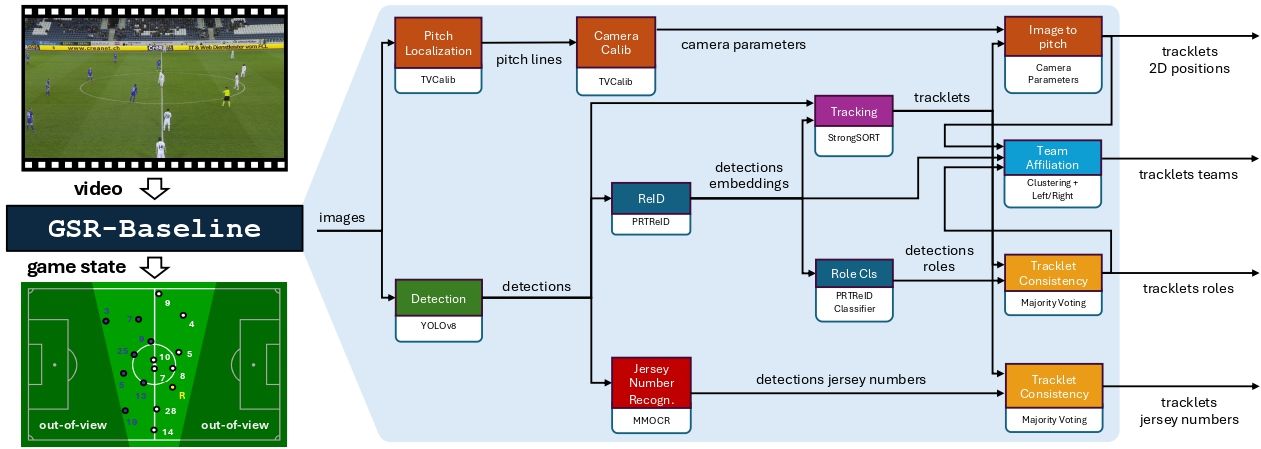
\includegraphics[width=\textwidth]{gsr_baseline_architecture.jpg}
    \caption{Arquitetura de referência do SoccerNet-GSR. Adaptado de \citet{somers2024soccernet}.}
    \label{fig:gsr-pipeline}
\end{figure}


Esta arquitetura modular tem, porém, um ponto fraco. O mapa só é útil se cada jogador estiver bem identificado, com o número da camisola, a equipa e a função certos, e não basta detetá-lo e segui-lo. Sem essa identificação, o mapa fica preenchido com posições sem identidade. As edições seguintes do desafio confirmam este diagnóstico \citep{cioppa2024soccernet, giancola2025soccernet}. A solução vencedora de 2024 \citep{golovkin2025minimap} segue, de forma independente, as duas ideias centrais desta dissertação. Na leitura do número, troca o OCR genérico por um modelo próprio para o futebol. Na equipa, junta a aparência à posição de cada jogador no campo. Há, no entanto, uma diferença de âmbito. Essa solução melhorou vários módulos ao mesmo tempo, da deteção à calibração, ao \emph{tracking} e ao pós-processamento. Esta dissertação altera apenas as duas tarefas de identificação. A deteção, o \emph{tracking} e a calibração ficam como na \emph{baseline}, e a reidentificação mantém o seu modelo, com um descritor de cor acrescentado para a atribuição da equipa. Assim, qualquer melhoria observada pode ser atribuída a estas alterações, e não a uma otimização global do sistema.

A reconstrução do estado de jogo é uma tarefa recente, disputada em apenas duas edições do desafio. Na primeira, em 2024, participaram dezasseis equipas com trinta e quatro submissões, e a solução vencedora elevou o GS-HOTA da \emph{baseline} de $23.36\%$ para $63.81\%$ \citep{cioppa2024soccernet}. Na segunda, em 2025, catorze equipas apresentaram sessenta e seis submissões sobre uma \emph{baseline} atualizada, com $29.01\%$, e a vencedora obteve $63.90\%$, com a solução vencedora de 2024 em segundo lugar, com o mesmo valor de $63.81\%$ \citep{giancola2025soccernet}. Deste historial, duas coisas contam para o que se segue. A primeira é que o valor máximo quase não se moveu entre as duas edições, apesar da mudança de paradigma na leitura do número, sinal de que a tarefa está longe de resolvida e de que nenhum módulo isolado a desbloqueia. A segunda é que os organizadores registam, na edição de 2025, três tendências comuns aos sistemas melhor classificados. São elas o recurso a características CLIP e OSNet para a reidentificação, a função e a equipa, o alisamento temporal da calibração por fluxo ótico, e a aplicação de modelos de visão e linguagem à leitura do número \citep{giancola2025soccernet}. A edição de 2026 do desafio já não incluiu a tarefa, substituída por cinco outras, entre as quais a deteção de ações centrada no jogador, que reutiliza a equipa e o número da camisola como identificadores \citep{cioppa2026soccernet}. Esta comparação é retomada no Capítulo~\ref{cap:resultados}, com a devida cautela, uma vez que o conjunto de teste usado neste trabalho não é o conjunto reservado em que o desafio apura as classificações.

\section{Reconhecimento do Número da Camisola}

O reconhecimento automático do número da camisola a partir de um vídeo de uma única câmara é difícil por razões que vêm da própria transmissão. A câmara está longe dos jogadores, e os algarismos ocupam poucos píxeis. Os jogadores correm, viram-se e tapam-se uns aos outros, e a camisola dobra-se com o movimento, pelo que o número raramente aparece de frente e legível. Os trabalhos publicados respondem a estas dificuldades de duas formas. Uns localizam e leem os dígitos em cada imagem, muitas vezes com a ajuda da pose. Outros aproveitam o facto de o mesmo jogador ser visto em muitas imagens e combinam as leituras ao longo do tempo. No fim da secção, descrevem-se as soluções apresentadas ao desafio SoccerNet.

\subsection{Abordagens por OCR Local e Modelos de Pose}

Os primeiros trabalhos abordaram a tarefa como um problema de deteção e classificação de dígitos. \citet{gerke2015soccer} foram dos primeiros a aplicar redes neuronais convolucionais (\emph{Convolutional Neural Networks}, CNN) ao reconhecimento do número da camisola, estabelecendo a viabilidade da abordagem. \citet{liu2019poseguided} deram um passo importante com uma R-CNN guiada por pose (\emph{pose-guided} R-CNN). Substituíram a \emph{Region Proposal Network} (RPN) tradicional por uma variante de três classes (fundo, pessoa e dígito) e usaram os \emph{keypoints} do corpo humano para refinar as propostas. Com isso, localizam melhor os dígitos, mesmo em poses difíceis. O modelo foi validado num conjunto de dados criado especificamente para o efeito, com anotações detalhadas de caixas de pessoa e de dígito.

Esta linha foi consolidada por \citet{liu2022jede} com o JEDE, um detetor universal que combina uma \emph{Feature Pyramid Network} (FPN) com uma \emph{Region Proposal Network} (RPN) e um ramo guiado por pose (\emph{pose-guided branch}) para as propostas de dígitos. Testado em futebol e basquetebol, superou métodos clássicos como o Faster R-CNN e o Mask TextSpotter, sobretudo na precisão e revocação da deteção.

Mais recentemente, \citet{koshkina2024general} propuseram uma abordagem distinta, que trata o reconhecimento do número como um caso de reconhecimento de texto em cena (\emph{scene text recognition}). Em vez de detetar cada dígito isoladamente, encadeiam um classificador de legibilidade (\emph{legibility classifier}), que descarta os \emph{frames} onde o número não está legível, com um modelo de reconhecimento de texto, agregando depois as leituras ao longo do \emph{tracklet}. Os autores disponibilizam ainda um conjunto de dados público, com anotações de legibilidade, e avaliam o desempenho tanto ao nível da imagem como do \emph{tracklet}. Ao escolher primeiro as imagens úteis e decidir depois ao longo do \emph{tracklet}, esta estratégia aproxima-se da adotada nesta dissertação. A diferença está nos meios. Os autores usam um classificador de legibilidade treinado à parte e um leitor de texto convencional. Este trabalho usa um modelo de visão e linguagem e a confiança que ele próprio atribui a cada leitura. Além disso, a abordagem dos autores é avaliada de forma isolada e num conjunto de dados próprio, e não dentro do \emph{pipeline} completo da reconstrução do estado de jogo.

\subsection{Abordagens temporais e por \emph{keyframes}}

Uma linha de investigação diferente tira partido do tempo, uma vez que a mesma camisola é vista em muitos \emph{frames}, mas só está legível em alguns. A ideia é escolher os bons em vez de ler todos. \citet{balaji2023jersey} apresentam uma rede espácio-temporal com um módulo que identifica os \emph{frames}-chave (\emph{keyframes}), aqueles em que o número aparece com mais nitidez, e concentram neles a leitura. O número é reconhecido por classificação, ou seja, a rede parte de uma lista fechada de números possíveis, fixada no treino, e escolhe um deles. É treinada com uma função de perda que junta num só objetivo a escolha dos \emph{keyframes} e o reconhecimento do número (\emph{multi-task loss}). A abordagem aguenta bem as oclusões e o movimento rápido, mas tem uma limitação que os próprios autores reconhecem, a de tratar o número como um todo, e não dígito a dígito.

O trabalho seguinte da mesma equipa, \citet{balaji2024dmae}, muda o foco. Em vez de escolher os melhores \emph{frames}, procura extrair de cada recorte características mais robustas, que aguentem a baixa resolução. Para isso recorre a um \emph{masked autoencoder}, uma rede que aprende sozinha, sem rótulos, tapando pedaços da imagem e treinando-se a reconstruí-los, o que a obriga a perceber a estrutura do que está a ver. O «\emph{domain-guided}» do nome vem de esse treino ser feito de propósito com imagens desfocadas por movimento, para se parecerem com as de uma transmissão real, e as leituras dos vários \emph{frames} são depois combinadas ao longo do tempo por um descodificador \emph{transformer}. Os ganhos que apresentam são modestos, mas reforçam a ideia que atravessa toda esta linha de trabalho. Em baixa resolução, a cor do equipamento não chega, e é preciso extrair da imagem características mais profundas para distinguir dígitos pequenos.

Nenhuma destas duas propostas foi seguida neste trabalho, e a razão é a mesma nas duas. Ambas assentam em modelos que é preciso treinar sobre imagens anotadas, o módulo de \emph{keyframes} num caso e o d-MAE no outro, e aqui não se treinou nenhum modelo nem se anotaram dados, até porque tudo tinha de encaixar na \emph{baseline} sem voltar a treinar as etapas anteriores. Ainda assim, a ideia que lhes está por trás, ler o número só onde ele se vê bem e juntar as leituras ao longo do tempo, é boa e foi aproveitada, mas por um caminho mais simples. Em vez de confiar a escolha dos \emph{frames} a um modelo treinado, escolhem-se em cada janela os recortes mais nítidos e contam só as leituras em que o próprio modelo se mostra seguro (Secção~\ref{sec:met-jnr}).

\subsection{Soluções submetidas ao desafio SoccerNet}\label{sec:jnr-desafio}

Os trabalhos analisados até aqui são artigos científicos, publicados e avaliados. Existe, porém, outro tipo de trabalho que não passa por essa avaliação, as soluções que concorreram às várias edições do desafio SoccerNet, descritas apenas nos relatórios oficiais. Para esta dissertação, são as fontes mais úteis. O que se extrai destas soluções não é apenas a classificação que alcançaram, mas também as escolhas técnicas que revelam. A leitura dos relatórios mostra, de forma geral, uma mudança do OCR tradicional para os modelos de visão e linguagem ao longo das três edições, de 2023 a 2025. As descrições que se seguem resumem o que as próprias equipas escreveram nesses relatórios \citep{cioppa2023soccernet, cioppa2024soccernet, giancola2025soccernet}, exceto quando se cita o artigo completo de uma delas.

Na edição de 2023, o reconhecimento do número foi disputado como uma tarefa à parte. Cada exemplo era um \emph{tracklet}, isto é, uma sequência de pequenos recortes do mesmo jogador retirada dos vídeos do SoccerNet-Tracking, e o objetivo era dizer que número, de 1 a 99, esse jogador tinha na camisola, ou responder $-1$ quando o número nunca chegava a ser visível. Os organizadores disponibilizaram 2853 \emph{tracklets} anotados, e a avaliação final foi feita sobre outros 1211, pela exatidão, ou seja, a percentagem de \emph{tracklets} com a resposta certa. Participaram quinze equipas, com 157 submissões, e a melhor chegou a $92{.}85\%$. Estes valores não são comparáveis com os desta dissertação. No desafio, os \emph{tracklets} já vinham feitos e só se media a leitura do número. Aqui, o número é um dos atributos do \emph{pipeline} completo, os \emph{tracklets} saem do próprio \emph{tracking}, com os seus erros, e a métrica é o GS-HOTA, que avalia ao mesmo tempo a deteção, o \emph{tracking} e a identificação de cada jogador.

Desta edição aproveita-se o método. Segundo os organizadores, a maioria das equipas resolveu o problema em três etapas. Primeiro, um detetor de texto, como o DBNet++, o MMOCR, o DeepSolo ou o YOLO, localiza o número em cada recorte. Depois, um modelo de OCR afinado para o efeito, tipicamente o PP-OCRv3 ou o PaddleOCR, lê o número identificado. Por fim, uma votação maioritária junta as leituras de todos os recortes do \emph{tracklet} em apenas uma resposta. A equipa vencedora seguiu o mesmo esquema e investiu sobretudo no treino. Usou o detetor de texto para retirar dos dados de treino as imagens sem número visível, aumentou esses dados com rotações, inversões, mudanças de escala, ruído e sobreposição de vários \emph{frames}, treinou cinco modelos de reconhecimento de texto diferentes e juntou os votos de todos. Daqui tiram-se duas lições. A primeira é que a votação ao longo do \emph{tracklet} já era prática corrente em 2023, e não é por isso uma novidade deste trabalho, que a aplica apenas às leituras em que o modelo está seguro. A segunda é que todas estas soluções dependem de afinar modelos de OCR com os \emph{tracklets} anotados do próprio desafio, e é precisamente esse treino que a abordagem da Secção~\ref{sec:met-jnr} dispensa.


Em 2024, na primeira edição da reconstrução do estado de jogo, o número deixou de ser uma tarefa à parte. Passou a ser um dos atributos que cada sistema tinha de identificar a partir dos seus próprios \emph{tracklets}. Viu-se assim uma mudança de abordagem, em que as equipas melhor classificadas trocaram o OCR genérico por modelos próprios, treinados só para o número da camisola.

\citet{golovkin2025minimap} dividem as soluções em dois grupos. O primeiro adapta técnicas de OCR de uso geral, que localizam o texto antes de o ler e perdem exatidão com jogadores distantes, com oclusões e com jogadores virados de lado. Já o segundo usa soluções desenhadas para o futebol, que são mais exatas, mas precisam de treino específico para cada conjunto de dados.

A solução vencedora, que é a dos próprios autores, é um bom exemplo do segundo grupo. Em vez de detetar cada dígito com uma caixa, usa uma rede residual modificada que recebe recortes de $32\times32$ píxeis e tem duas cabeças de classificação, uma que prevê o algarismo das dezenas, ou que ele não existe, e outra que prevê o das unidades. Assim, consegue ler o número mesmo quando parte dele está tapada, e não é preciso anotar uma caixa à volta de cada dígito. A equipa UPCxMobius, com a solução \emph{No bells, More Whistles}, que ficou em segundo lugar \citep[equipa GSR-2]{cioppa2024soccernet}, seguiu um caminho parecido e treinou um detetor de dígitos com dados públicos e cerca de mil \emph{frames} anotados de propósito. A equipa \emph{playbox x NUSG} \citep[equipa GSR-14]{cioppa2024soccernet} usou o CLIP em duas fases, com um modelo a decidir se há número visível e outro a dizer qual é, afinados sobre três mil caixas anotadas à mão, mas no conjunto final do desafio não chegou a superar a \emph{baseline}. O que estas soluções têm em comum é o custo de anotação. Cada uma teve de construir o seu próprio conjunto de treino, um esforço que as condições desta dissertação não permitiam.

A edição de 2025 marca uma mudança clara. Os organizadores referem, no relatório final dos resultados, que os modelos de visão e linguagem foram aplicados com sucesso à leitura do número. Destacam o LLaMA-3.2-Vision \citep{grattafiori2024llama3} e o Qwen2-VL-Instruct \citep{wang2024qwen2vl}. O primeiro foi utilizado pela equipa vencedora, a KIST \citep[equipa GSR-1]{giancola2025soccernet}, cujo sistema é descrito em detalhe por \citet{oo2026broadcast2pitch}. Os autores tratam a identificação completa do jogador como uma tarefa de geração autorregressiva multimodal. Em vez de treinarem um classificador por atributo, dão ao modelo o recorte do jogador com uma instrução em linguagem natural que lhe pede a função, o número e a cor da camisola, e leem a resposta como uma sequência de \emph{tokens}. Justificam a escolha com três vantagens. A primeira é generalizar melhor a atributos nunca vistos, como cores de camisola novas, o que é essencial para um reconhecimento aberto. A segunda é exigir menos anotação e menos engenharia, porque basta ajustar a instrução para pedir outras tarefas, sem mudar a arquitetura. A terceira é poder adaptar-se a outros ambientes desportivos e formatos de jogo. O Qwen2-VL-Instruct foi usado de outra forma pela equipa eidos.ai, sétima classificada \citep[equipa GSR-7]{giancola2025soccernet}. Em vez de classificar cada deteção à parte, mostra ao modelo uma longa sequência de deteções organizadas numa grelha e pede-lhe que raciocine passo a passo antes de responder.

O artigo de \citet{oo2026broadcast2pitch} traz ainda a comparação mais direta entre abordagens encontrada na literatura, porque testa três modelos de identificação dentro do mesmo \emph{pipeline} e sobre o mesmo conjunto de teste. Como primeira abordagem, junta modelos especializados por atributo, o PRTreID para a função, o EasyOCR para o número e uma ResNet-18 para a cor da camisola, e com isso obtém $18{.}11\%$ de GS-HOTA. Já a segunda abordagem usa o CLIP como codificador, com uma cabeça de classificação para cada atributo, e chega a $60{.}13\%$. Por fim, a terceira abordagem, com o LLaMA-3.2-Vision, sobe ligeiramente para $61{.}48\%$. Como o resto do sistema é igual nas três configurações, a diferença vem só do módulo de identificação. Não se pode atribuir apenas ao número, porque esse módulo decide também a função e a equipa, mas uma distância de mais de quarenta pontos deixa claro que os modelos de visão e linguagem identificam o jogador muito melhor do que um conjunto de modelos separados. Os autores reconhecem, ainda assim, que a vantagem do LLaMA-3.2-Vision sobre o CLIP é pequena e tem um custo computacional maior. Em sentido contrário, a equipa Playbox \& MIXI, quarta classificada \citep[equipa GSR-4]{giancola2025soccernet}, manteve o reconhecimento de texto convencional. Isola primeiro o tronco do jogador com os pontos do ViTPose e só depois lê o número com o PARSeq, os mesmos passos do método de \citet{koshkina2024general}. É a ideia de recorte orientado pela pose que este trabalho também usa (Secção~\ref{sec:met-jnr}), aqui ligada a um OCR clássico, o que indica que o OCR ainda tem lugar entre os melhores sistemas quando recebe a região certa da camisola.

Mais do que um trabalho aponta o número da camisola como o atributo mais difícil de todo o sistema. Por exemplo, a UTokyo Football Lab, da Universidade de Tóquio \citep[equipa GSR-8]{giancola2025soccernet}, termina a sua descrição a reconhecer que, tal como na \emph{baseline}, a maior dificuldade esteve no reconhecimento do número, e aponta os modelos multimodais como o passo seguinte. A prova mais completa vem, outra vez, de \citet{oo2026broadcast2pitch}, que calculam a métrica oficial juntando um atributo de cada vez à posição, dentro do seu próprio sistema. Só com a posição no campo, o GS-HOTA chega a $79{.}52\%$. Com a função, quase não muda e fica em $79{.}20\%$. Com a equipa, desce para $73{.}58\%$, ou para $77{.}39\%$ sem três vídeos em que a equipa está mal anotada. Com o número da camisola, cai para $64{.}70\%$, e com todos os atributos juntos fica em $61{.}48\%$. O número é, portanto, o atributo que mais custa ao sistema, com uma perda de quase quinze pontos. Os autores explicam-no pela própria transmissão televisiva, em que os dígitos aparecem desfocados, tapados ou visíveis em poucos \emph{frames} de cada \emph{tracklet}. Acrescentam que a votação maioritária por \emph{tracklet} se torna frágil quando as leituras certas são poucas, problema que a votação restrita às leituras seguras procura atenuar (Secção~\ref{sec:met-jnr}). É uma confirmação externa, e com números, da premissa de que esta dissertação parte. Nos mesmos dados, a equipa é o segundo atributo que mais custa, bem à frente da função, o que justifica que sejam o número e a equipa os dois atributos em que este trabalho intervém.


\section{Atribuição da equipa}

A atribuição da equipa consiste em decidir a que equipa cada jogador pertence. Na maior parte dos trabalhos, essa decisão faz-se com base na aparência, seja pela cor do equipamento, seja por características aprendidas por uma rede neuronal. Os métodos diferenciam-se sobretudo pela informação que usam para separar as duas equipas. 
Na reconstrução do estado de jogo há ainda um segundo passo, pois não é suficiente separar os jogadores em dois grupos. Também é necessário determinar qual das equipas defende a baliza da esquerda e qual defende a da direita. As subsecções seguintes começam pelos métodos baseados na cor, passam pelos que aprendem as características a partir dos dados e terminam nas soluções submetidas ao desafio SoccerNet, onde surge a questão do lado do campo.
\subsection{Métodos baseados em cor}

Os métodos mais simples usam a cor do equipamento para separar as equipas. As próprias Leis do Jogo ajudam nesta tarefa, pois obrigam as duas equipas a vestir cores que as distingam uma da outra e da equipa de arbitragem. Por isso, para quem vê o jogo, a cor chega quase sempre para distinguir as duas equipas. A exceção é o guarda-redes, que tem de usar uma cor diferente da de todos os outros jogadores, incluindo os da sua própria equipa. Assim, só pela cor, não há forma de saber a que equipa ele pertence. Num sistema automático, a cor é menos fiável do que parece, porque a mesma camisola muda de tom com a luz e a sombra, fica desfocada quando o jogador corre e, nos jogadores mais distantes, ocupa poucos píxeis.

O DeepPlayer-Track, de \citet{naik2022deepplayer}, mostra como esta abordagem funciona na prática. Cada jogador detetado é atribuído a uma das equipas, ou ao árbitro, apenas pela cor da camisola, e essa atribuição é depois usada para seguir os jogadores ao longo do vídeo sem que troquem de identidade. É um caso útil para esta dissertação por duas razões. Foi testado, entre outros, em transmissões televisivas do SoccerNet, o mesmo tipo de vídeo usado neste trabalho, e os autores mostram, com exemplos, onde a separação pela cor falha. O sistema funciona em duas etapas. Na primeira, um detetor YOLOv4 encontra em cada \emph{frame} os jogadores, a bola e o árbitro, e trata como fundo tudo o que está fora do campo. Na segunda, cada caixa é classificada pela cor, comparando os seus píxeis com três gamas de cor que os autores escolheram à mão a partir dos próprios vídeos, uma para a equipa de branco, outra para a de azul e outra para o árbitro, de vermelho. Essa classificação entra depois no \emph{tracker}, o JCD-SORT, uma variante do SORT. Para decidir a que trajetória pertence cada nova deteção, o \emph{tracker} combina a cor com a distância do cosseno entre descritores de aparência extraídos por uma rede convolucional. Com isso, dois jogadores de equipas diferentes dificilmente trocam de identidade, mesmo quando se cruzam.

O trabalho mostra que, com as gamas certas, a cor chega para separar as duas equipas e o árbitro. O ponto fraco está em essas gamas serem escolhidas à mão e só servirem nos vídeos em que foram escolhidas. Os próprios autores apresentam um vídeo do SoccerNet em que o árbitro não veste de vermelho, e o sistema, que só o reconhece por essa cor, trata-o como mais um jogador. Reconhecem também que a cor não resolve as trocas entre jogadores da mesma equipa, que continuam a acontecer quando um tapa o outro, e propõem, como trabalho futuro, reconhecer o número da camisola para os distinguir. Um método com as cores definidas à partida tem, portanto, de ser reconfigurado para cada jogo e falha sempre que alguém em campo vestir uma cor que não estava prevista. É precisamente essa configuração manual que este trabalho pretende evitar.

O PlayerTV, de \citet{solberg2024playertv}, reduz essa configuração ao mínimo e combina a cor com outra característica do jogador. Este sistema gera automaticamente resumos com os lances de cada jogador e, para isso, precisa de saber a equipa e o número de cada um. A equipa vem da cor, mas sem gamas fixas. Para cada \emph{tracklet}, calcula-se a cor média de uma região da metade de cima do jogador, cortando os lados para deixar de fora a relva. Essas cores são divididas em dois grupos pelo \emph{k-means}, e cada \emph{tracklet} fica na equipa do grupo mais próximo. Os grupos são aprendidos em cada vídeo, e a única informação de cor dada à partida é uma base de dados com as cores do equipamento principal e alternativo de cada equipa da liga, que serve apenas para dar nome a cada grupo. Essa outra característica é o número da camisola. Quando o número lido é mais seguro do que a cor, e ainda não está atribuído na outra equipa, é o número que decide a equipa. Em 16 vídeos da liga norueguesa, com 511 \emph{tracklets} anotados, a equipa fica certa em $91{.}5\%$ dos casos no espaço de cor CIELAB, e em $93{.}7\%$ depois do pós-processamento. O número, pelo contrário, só é lido corretamente em cerca de $30\%$ dos \emph{tracklets}, e os autores apontam-no como a principal limitação do sistema. Por procurar apenas dois grupos, um para cada equipa, o método também não identifica o árbitro.

Já \citet{pan2024unsupervised} vão mais longe e usam apenas a cor, sem nenhuma informação dada à partida, num método avaliado no SoccerNet-GSR, o mesmo conjunto de dados desta dissertação. O problema de que tratam é o da luz, porque nos jogos ao ar livre a mesma camisola pode parecer de duas cores diferentes conforme o jogador está ao sol ou à sombra. Por isso, antes de agrupar as pessoas pelas suas cores dominantes, o método corrige as sombras da imagem. No SoccerNet-GSR, chega a uma exatidão de $85{.}4\%$. Os próprios autores reconhecem, no entanto, duas limitações. Os grupos são formados imagem a imagem, sem ligação ao longo do vídeo, e o método ainda não chega aos cinco papéis que pretendem, as duas equipas, os dois guarda-redes e o árbitro, para o que propõem juntar à cor a posição dos jogadores no campo.

Os três trabalhos mostram que a cor separa bem as equipas. O que muda de um para o outro é quanto é preciso configurar à mão. O DeepPlayer-Track precisa de gamas de cor escolhidas para cada jogo. O PlayerTV aprende os grupos em cada vídeo, mas usa uma base de dados para lhes dar nome. O método de \citet{pan2024unsupervised} dispensa as duas coisas. Nenhum deles resolve, no entanto, o guarda-redes, e nenhum chega ao segundo passo, o de dizer que equipa defende cada baliza. O PlayerTV deixa ainda uma confirmação útil para esta dissertação. Com uma solução tão simples como a cor média, a equipa fica certa em mais de $90\%$ dos \emph{tracklets}, mas o número da camisola fica pelos $30\%$, o que volta a mostrar que é no número que está a maior dificuldade. Este trabalho segue a mesma ideia de aprender a separação em cada vídeo, sem nada configurado à mão, mas com características aprendidas em vez da cor, o tipo de abordagem tratado na subsecção seguinte.

\subsection{Métodos por aprendizagem e agrupamento}

Para ganhar robustez, outros trabalhos substituem a cor por características aprendidas por redes neuronais. A ideia comum é representar cada jogador por um vetor de características, de modo que a distância entre jogadores de equipas diferentes seja maior do que entre jogadores da mesma equipa. A rede é treinada uma única vez, e em cada jogo basta agrupar esses vetores, o que permite lidar com equipas e equipamentos que a rede nunca viu. Os trabalhos distinguem-se sobretudo no modo como essa representação é aprendida.

O trabalho de \citet{alhejaily2023team} é o exemplo mais simples destes métodos, porque a rede não é treinada para separar equipas. Os autores usam um \emph{autoencoder} convolucional, uma rede com duas metades. A primeira resume a imagem num vetor pequeno, e a segunda tenta reconstruir a imagem original apenas a partir desse vetor. O treino consiste em comparar a imagem reconstruída com a original e em corrigir a rede para que fiquem cada vez mais parecidas, o que dispensa qualquer rótulo. A rede é treinada uma vez sobre o Tiny ImageNet, um conjunto de imagens genéricas que nem sequer são de futebol. Depois de treinada, usa-se só a primeira metade, para transformar o recorte de cada pessoa num vetor, e a separação das equipas fica a cargo do \emph{k-means}, refeito em cada vídeo. Para isso, os autores escolhem 100 \emph{frames} ao acaso, detetam as pessoas com um detetor YOLOv3, passam cada recorte pela rede e dividem os vetores resultantes em três grupos, um para cada equipa e um terceiro para os guarda-redes e os árbitros. A partir daí, cada jogador fica no grupo cujo centro está mais próximo do seu vetor. Em 100 \emph{frames} anotados à mão, o método acerta em $92\%$ dos casos. Com o mesmo \emph{k-means} aplicado diretamente às cores dos recortes, acerta em $86\%$. A vantagem é não precisar de nenhum dado de futebol anotado. O preço é que o vetor guarda tudo o que é preciso para reconstruir a imagem, incluindo a luz e a sombra, e não apenas o que distingue as equipas. \citet{pan2024unsupervised} mostram precisamente que, com luz irregular, este método pode pôr os jogadores que estão à sombra num grupo à parte.

\citet{istasse2019associative} seguem o caminho oposto e treinam a rede precisamente para separar equipas, em imagens de basquetebol. A rede trabalha sobre a imagem inteira, e não sobre recortes de jogadores. Segmenta os jogadores, tratando os árbitros como fundo, e atribui a cada píxel um vetor, aprendido de modo a ser parecido entre jogadores da mesma equipa e diferente entre as duas equipas da mesma imagem. Como aprende a separar as equipas presentes em cada imagem, e não a reconhecer cores concretas, não precisa de ser treinada de novo para cada jogo, embora o treino inicial exija imagens anotadas com a equipa de cada jogador. Em jogos e pavilhões que não viu no treino, atribui a equipa certa a mais de $90\%$ dos jogadores, contra $62\%$ de um agrupamento por histogramas de cor. A decisão é, no entanto, tomada imagem a imagem, sem \emph{tracklets} nem ligação entre imagens seguidas do vídeo.

\citet{koshkina2021contrastive} treinam uma representação do mesmo tipo sem nenhum rótulo de equipa, em vídeos de hóquei no gelo filmados por uma câmara fixa que apanha o rinque inteiro. Usam aprendizagem contrastiva (\emph{contrastive learning}), em que a rede aprende a aproximar exemplos do mesmo grupo e a afastar os de grupos diferentes. Como não há rótulos, os grupos de partida vêm da cor, e só os jogadores agrupados com mais segurança servem de exemplos para o treino. Ao contrário do trabalho anterior, a rede trabalha sobre o recorte de cada jogador detetado. Num jogo novo, os recortes dos primeiros \emph{frames} chegam para encontrar os centros das duas equipas, e a partir daí cada jogador detetado fica na equipa do centro mais próximo. Com um único \emph{frame}, a equipa fica certa em $94\%$ dos casos, e com 500 \emph{frames}, cerca de 17 segundos de jogo, em $97\%$. O árbitro é identificado à parte, por um classificador treinado com exemplos anotados. Tal como no trabalho anterior, não há \emph{tracklets}, e cada deteção é decidida isoladamente.

A mesma ideia está no PRTreID, de \citet{mansourian2023multitask}, a rede cujas representações a \emph{baseline} usa para atribuir a equipa. O PRTreID é uma rede de reidentificação, treinada com recortes de jogadores do SoccerNet, que aprende três tarefas ao mesmo tempo. Reconhece a mesma pessoa em imagens diferentes, classifica a sua função e separa as equipas. Na tarefa da equipa, todos os recortes de cada lote de treino vêm do mesmo vídeo, e a rede aprende a aproximar jogadores da mesma equipa e a afastar os da equipa adversária. Tal como em \citet{istasse2019associative}, a comparação faz-se sempre dentro do mesmo jogo, e por isso a rede não aprende nenhuma equipa em concreto e pode ser usada em qualquer jogo. Esta tarefa usa apenas jogadores de campo, ficando de fora os guarda-redes, os árbitros e os restantes elementos. Os autores medem o seu efeito dividindo os jogadores de cada vídeo em dois grupos pelo \emph{k-means}. Com a rede treinada só para reidentificação, a equipa fica certa em $91{.}87\%$ dos casos, e com as três tarefas em conjunto sobe para $95{.}6\%$.

A \emph{baseline} \citep{somers2024soccernet} usa estas representações com uma diferença importante em relação aos trabalhos desta subsecção. Em vez de decidir a equipa imagem a imagem ou deteção a deteção, decide-a por \emph{tracklet}. Para cada \emph{tracklet} com a função de jogador, faz-se a média das representações do PRTreID de todas as suas deteções, o que dá um único vetor por \emph{tracklet}. Esses vetores são divididos em dois grupos pelo \emph{k-means}, e todas as deteções de um \emph{tracklet} recebem a equipa do seu grupo. Por fim, o lado de cada grupo decide-se pela posição média dos seus jogadores no campo, um passo que se discute na subsecção seguinte.

Os vetores de características aprendidos por uma rede neuronal separam melhor as equipas do que a cor, como mostram as comparações de \citet{alhejaily2023team}, com $92\%$ contra $86\%$, e de \citet{istasse2019associative}, com $90\%$ contra $62\%$. Todos estes métodos tratam, no entanto, o guarda-redes e o árbitro à parte, e só a \emph{baseline} decide por \emph{tracklet} e chega ao lado do campo. Este trabalho parte dessa mesma base, os vetores do PRTreID agrupados por \emph{tracklet} em cada vídeo, e recorre à cor apenas nos vídeos em que esses vetores não separam bem as duas equipas, como se descreve no Capítulo~\ref{cap:metodologia}.

\subsection{Soluções submetidas ao desafio SoccerNet}\label{sec:equipa-desafio}

Ao contrário da maioria dos trabalhos anteriores, as soluções submetidas ao desafio têm de resolver os dois passos, porque a métrica oficial exige que cada jogador seja identificado como pertencendo à equipa da esquerda ou à da direita. Esta subsecção descreve primeiro como separam as equipas e depois como decidem o lado, que é onde mais divergem.

Para o primeiro passo, \citet{golovkin2025minimap} descrevem uma estrutura comum à maioria dos sistemas, a mesma das subsecções anteriores. Cada jogador é descrito por um histograma de cor ou por um vetor de reidentificação, e esses vetores são agrupados pelo \emph{k-means} ou pelo DBSCAN em dois a cinco grupos, conforme se separam só as duas equipas ou também os árbitros e os guarda-redes. A solução vencedora de 2024, que é a dos próprios autores, segue esta estrutura com dois cuidados. Os vetores vêm de uma OSNet treinada para distinguir 111 equipamentos diferentes, e os grupos são cinco, as duas equipas, os árbitros e os dois guarda-redes. Para estimar os grupos das equipas e dos árbitros, usam apenas os jogadores a menos de 30 metros do centro do campo, o que deixa de fora os guarda-redes. Estes são procurados depois dentro de cada grande área.

Em 2025 aparecem duas orientações diferentes. A vencedora, a KIST \citep[equipa GSR-1]{giancola2025soccernet}, entrega a tarefa ao mesmo modelo de visão e linguagem que lê o número. O LLaMA-3.2-Vision devolve a cor do equipamento de cada jogador, e as equipas obtêm-se agrupando essas cores \citep{oo2026broadcast2pitch}. A UTokyo Football Lab \citep[equipa GSR-8]{giancola2025soccernet} reforça, pelo contrário, a informação de aparência. Segmenta a silhueta de cada jogador e extrai dela um vetor de dez dimensões com as cores do equipamento e as respetivas áreas, que junta às entradas dos módulos de reidentificação, de função e de equipa.

A equipa que ficou em último lugar em 2024, a eidos.ai \citep[equipa GSR-16]{cioppa2024soccernet}, a mesma que em 2025 usou o Qwen2-VL para o número, também deixa uma lição. Tentou resolver a função e a equipa de uma só vez para todo o vídeo, com uma rede siamesa que produz os vetores, um \emph{k-means} corrido com vários números de grupos e uma floresta aleatória que escolhe o agrupamento mais plausível a partir de informação de contexto do jogo. Ficou com $8{.}92\%$ de GS-HOTA, contra $23{.}36\%$ da \emph{baseline}, e os autores consideram provável que a causa seja terem treinado o modelo com as posições da anotação e o terem avaliado com as deteções reais. É um exemplo claro de como os erros das etapas anteriores condicionam tudo o que vem depois.

Separadas as equipas, falta decidir que grupo defende cada baliza. A regra mais comum compara a posição horizontal média dos jogadores de cada grupo e dá o lado direito ao grupo cuja média está mais à direita. É o que faz a \emph{baseline} e também a vencedora de 2025, que assume que os jogadores tendem a ficar mais perto da sua metade do campo. Os próprios autores reconhecem que esta suposição pode falhar em cantos ou em períodos longos de pressão alta \citep{oo2026broadcast2pitch}. O trabalho vencedor de 2024 troca a média única por uma votação, em que em cada \emph{frame} se compara a posição média dos dois grupos e se regista qual está mais à direita. Justifica a alteração com o facto de a média ao longo de todo o vídeo poder falhar em vídeos muito curtos ou quando só parte do campo está visível.

O guarda-redes é outra pista usada. A vencedora de 2024 procura-o dentro de cada grande área, e a Playbox \& MIXI \citep[equipa GSR-4]{giancola2025soccernet} atribui a função de guarda-redes ao jogador mais afastado dentro de cada área, corrigindo depois o resultado com uma otimização que penaliza configurações impossíveis, como a existência de vários guarda-redes. Identificar o guarda-redes pela posição não é, portanto, original deste trabalho, que o usa apenas como último critério de desempate do lado (Secção~\ref{sec:mapeamento}).

Falta, ainda assim, saber com que frequência a regra da posição média falha. As vencedoras de 2024 e de 2025 apontam situações em que isso acontece, mas nenhuma conta os casos. A única avaliação isolada desta etapa é a da própria \emph{baseline} \citep{somers2024soccernet}. Com todas as outras etapas substituídas pela anotação, a regra do lado obtém $92\%$ de GS-HOTA, e os autores concluem que é muito eficaz. Essa medida parte, porém, de \emph{tracklets} e equipas perfeitos, e não diz quantos vídeos ficam com os lados trocados nem o que acontece quando os grupos vêm do próprio sistema. O Capítulo~\ref{cap:resultados} responde às duas questões. Mede, sobre a anotação dos $160$ vídeos, com que frequência a regra da posição média discorda do lado anotado. Conta depois, entre os $159$ processados pelos dois sistemas, quantos ficam com o lado trocado.

\section{Métricas de Avaliação}\label{sec:metricas}

Avaliar a reconstrução do estado de jogo obriga a medir duas coisas ao mesmo tempo. É preciso saber se cada jogador foi localizado no sítio certo do campo e se foi identificado corretamente, com a função, a equipa e o número da camisola certos. A métrica oficial do desafio, o GS-HOTA, foi proposta por \citet{somers2024soccernet} juntamente com a própria tarefa, para medir as duas coisas numa só. Parte do HOTA \citep{luiten2021hota}, uma métrica de \emph{tracking} de múltiplos objetos que combina a qualidade da deteção com a da associação ao longo do tempo, e muda a forma de comparar cada previsão com a anotação. A semelhança entre as duas passa a ser o produto de dois termos. O primeiro depende da distância no campo, e a partir de $5$ metros a previsão já não pode ser associada a esse jogador. O segundo vale $1$ se todos os atributos estiverem certos e $0$ se algum estiver errado. Na prática, um jogador bem localizado, mas com a equipa ou o número errados, deixa de poder ser associado ao jogador real e conta duas vezes como erro, como jogador em falta e como deteção a mais. É isto que torna o GS-HOTA tão exigente com os atributos estudados nesta dissertação.

Por ser uma métrica única para todo o sistema, o GS-HOTA mistura os erros de todos os módulos, da deteção e do \emph{tracking} à calibração e aos atributos, e não diz qual deles pesa mais. Os próprios autores da métrica mostram como separar esse peso, calculando-a com os atributos ligados progressivamente, primeiro só a posição e depois a função, a equipa e o número \citep{somers2024soccernet}. A diferença entre dois cálculos seguidos dá o custo de cada atributo. É o mesmo procedimento usado por \citet{oo2026broadcast2pitch} e retomado no Capítulo~\ref{cap:resultados}. Para medir cada módulo isoladamente, usa-se ainda a exatidão por \emph{tracklet}, isto é, a percentagem de \emph{tracklets} com o número certo, ou com a equipa e o lado certos, a mesma medida que o desafio de 2023 usava para o número. As duas medidas completam-se. O GS-HOTA mostra o efeito de cada alteração no sistema completo e permite a comparação com o desafio, e a exatidão por \emph{tracklet} mostra o que mudou em cada módulo.

\section{Síntese e Lacunas Identificadas}
\label{sec:sintese_lacunas}

O estado da arte revisto mostra duas evoluções. No número da camisola, os métodos passaram de detetores e leitores de texto treinados com dados anotados para modelos de visão e linguagem, que em 2025 estiveram na base da solução vencedora. Na equipa, a cor do equipamento continua a ser um bom ponto de partida, mas os métodos mais robustos aprendem vetores de características e agrupam-nos em cada jogo, como faz a \emph{baseline} com o PRTreID. Da comparação destes trabalhos com as soluções do desafio resultam três lacunas, que motivam o presente trabalho:

\begin{enumerate}
    \item \textbf{O número continua a ser o ponto fraco.} O próprio artigo da \emph{baseline} aponta o número como a sua maior dificuldade, à frente da localização no campo e da equipa \citep{somers2024soccernet}, e o mesmo diagnóstico aparece nas soluções do desafio. Mesmo no sistema vencedor de 2025, o número é o atributo que mais custa, quase quinze pontos de GS-HOTA \citep{oo2026broadcast2pitch}. Os melhores resultados exigem, além disso, modelos pesados. A equipa vencedora afina o LLaMA-3.2-Vision com os dados do SoccerNet e corre-o numa placa gráfica de 24 GB, e os próprios autores apontam o custo computacional como uma limitação.

    \item \textbf{O lado do campo nunca foi medido em condições reais.} A regra da posição média, usada pela \emph{baseline} e pela equipa vencedora de 2025, falha em situações que as próprias equipas vencedoras de 2024 e de 2025 descrevem, mas ninguém conta esses casos. A única avaliação isolada desta etapa usa \emph{tracklets} e equipas perfeitos, tirados da anotação \citep{somers2024soccernet}.

    \item \textbf{Os ganhos não se conseguem atribuir.} Os trabalhos académicos avaliam os seus métodos isoladamente, muitas vezes em conjuntos de dados próprios, fora de um \emph{pipeline} completo e sem a métrica oficial. As soluções do desafio são avaliadas no \emph{pipeline} completo, mas alteram muitos módulos ao mesmo tempo, e o ganho em relação à \emph{baseline} mistura todas as alterações. \citet{oo2026broadcast2pitch} comparam três modelos de identificação dentro do seu sistema, mas esse sistema já tem o \emph{tracking} e a calibração alterados.
\end{enumerate}

A terceira lacuna define a estratégia experimental deste trabalho, e as duas primeiras definem o seu âmbito. Só se alteram o reconhecimento do número e a atribuição da equipa e do lado. A deteção, o \emph{tracking}, a calibração e o modelo de reidentificação ficam exatamente como na \emph{baseline}. Assim, qualquer diferença de desempenho resulta apenas do que foi alterado. O trabalho segue a mesma direção das soluções mais competitivas no uso de um modelo de visão e linguagem para o número, mas com um modelo mais pequeno, o Qwen2.5-VL-3B quantizado a 4 bits, sem qualquer treino e numa placa gráfica de 6 GB.
